% ----------------------------------------------------------
% PARTE
% ----------------------------------------------------------
\part{Resultados}
% ----------------------------------------------------------

\section{Kaggle}

Kaggle é uma plataforma criada em 2010 que reune ferramentas e estudos sobre modelagem preditiva. Também viabiliza competições de temas relacionados a análise preditiva. Com o intuito de compartilhar conhecimento, qualquer interessado pode acessar dados de empresas para aplicar estudos ou gerar novos modelos. Além disso, o Kaggle também tem sido usado como uma forma de recrutar cientistas de dados. 


\subsection{Loan Club}

A Loan Club é um marketplace de créditos online. Trata-se de uma plataforma que reune pessoas que gostaria de realizar um empréstimo e outras que possuem um capital a investir. Em geral, são empréstimos pessoas, de negócios ou para procedimentos médicos. A proposta é oferecer um serviço de fácil acesso via dispositivos mobiles a taxa baixas, além de garantir um retorno que se ajuste a expectativa do investidor. Dessa forma, operam de forma menos burocrática do que um banco, mas assumindo os riscos de uma instituição financeira.


\section{Tecnologias}

\subsection{Scikit Learn}

O scikit é um framework desenvolvido em Python voltado para data science. Possui implementação de diversos algoritmos e de ferramentas que auxiliam desde a análise dos dados até na execução de tarefas como clusterização e classificação até a execução dos algoritmos de machine learning. Possui integrações com programas visuais (como será mostrado a seguir). Já são mais de 30 contribuidores ativos.


\subsection{Apache Spark}

O Apache Spark é uma ferramenta que resolve um problema relacionado a escalabilidade da execução de algoritmos de machine learning. Os 3 algoritmos estudos (em especial o Kmédias) possui uma carga de contas alto. Para bases grandes, aspecto relevante quando se trata de Big Data, o scikit não é capaz de executar em tempo hábil. O Apache Spark, por outro lado, oferece uma solução robusta para a execução dos algoritmos de machine learning. Embora seja possível configurá-lo para que os algortimos sejam executados em tempo real com alimentação contínua de dados, tal abordagem não será contemplada por não se tratar do foco do estudo.

\section{Algoritmos}

\subsection{Preparação da base}

Como uma base de uma empresa, o Loan Club apresenta diversos problemas como:

- Missing values
Ocorre quando uma informação não consta na base. Esse fato influencia na conclusão de uma análise porque é necessário verificar a natureza da informação. Elas são oriundas desde problemas ao guardar a informação (como erro humano, falta de informação ou em decorrência de algum problema ou inconsistência no sistema que armazenou). Para os algortimos, é necessário que algum valor seja colocado para a realização das cálculos dos algoritmos. Nessas situações, existem abordagens diferentes, como subustituição por um valor padrão que faça sentido. Em alguns casos, são usados valores considerado neutros como 0, média ou moda das observações. Contido, é evidente que cada uma dessas técnicas enviesa e modifica o resultado. Para essa situação, neste estudo, desprezamos as informações que possuiam altas ocorrências de missing values.

- Necessidade de tratamentos de dados
Foram realizados 3 transformações: normalização de dados para o k médias, tratamento de dados de texto para valores (completar) e remoção das variáveis categóricas.

\subsection{K Médias}

PS: perguntar sobre normalização

No diagrama de Vorogorov é possível ter uma visualização espacial da distribuição dos registros, bem como os centróides.

\begin{figure}[!ht]
\caption{Visualização dos pontos no diagrama de Vorogorov }
\centerline{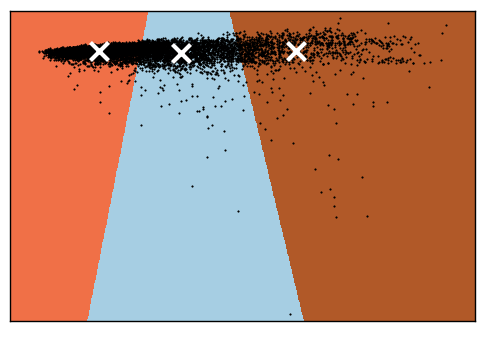
\includegraphics[width=0.5\textwidth]{img/voronoi}}
\fonte{Gerado a partir do script}
\end{figure}

 Para isso, foi necessário realizar uma operação de redução de dimensionalidade de veriáveis para 2 features. Neste estudo, aplicamos a construção do diagrama para 8000 registros.


Também é possível fazer uma análise para verificar a quantidade de clusters ideal para a amostragem.

\begin{figure}[!ht]
\caption{Analise para 2 clusters }
\centerline{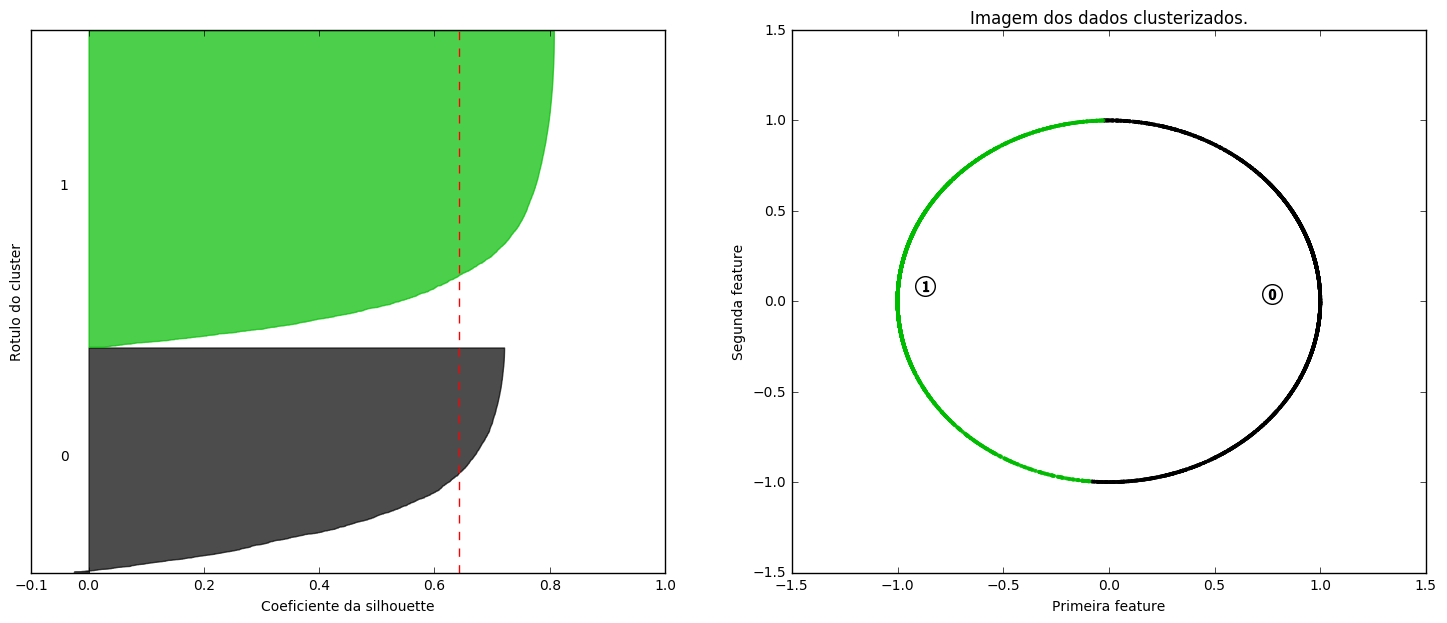
\includegraphics[width=1\textwidth]{img/silhoute2}}
\fonte{Gerado a partir do script}
\end{figure}

Para a divisão em 2 clusters, foi obtida a nota 0,5516

\begin{figure}[!ht]
\caption{Analise dos 3 clusters }
\centerline{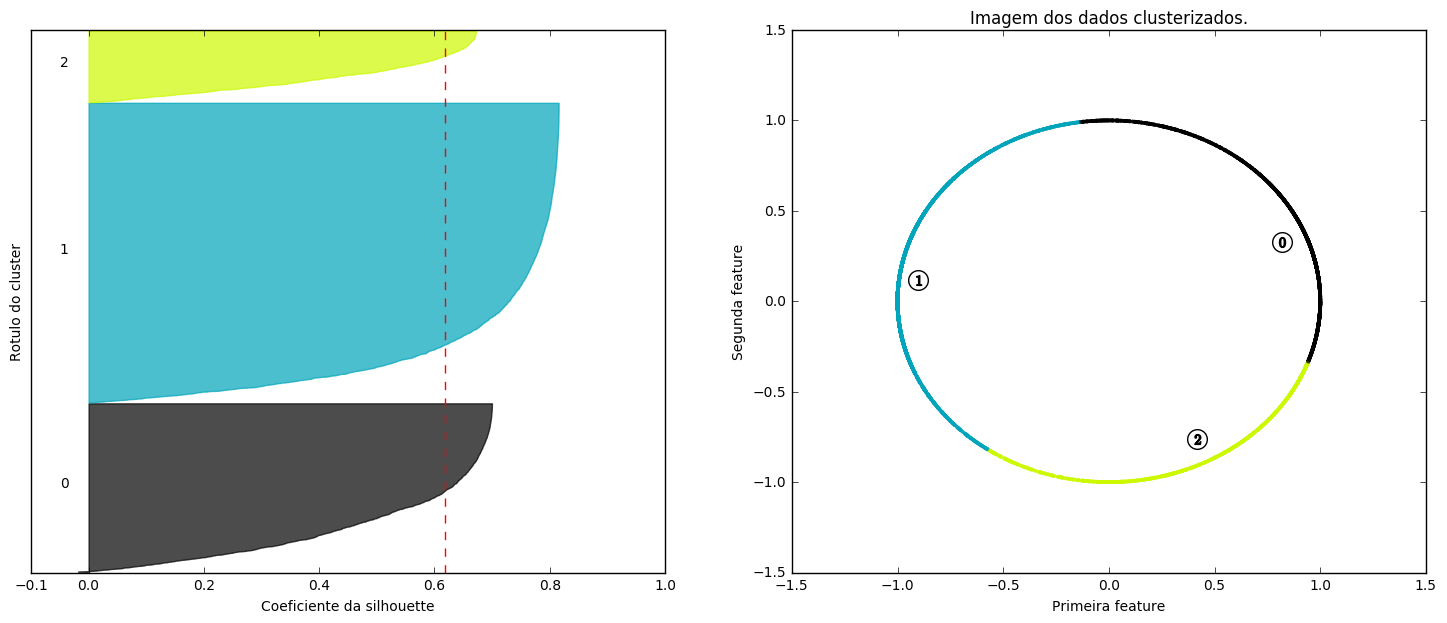
\includegraphics[width=1\textwidth]{img/silhoute3}}
\fonte{Gerado a partir do script}
\end{figure}

Para a divisão em 3 clusters, foi obtida a nota 0,4463

\begin{figure}[!ht]
\caption{Analise dos 4 clusters }
\centerline{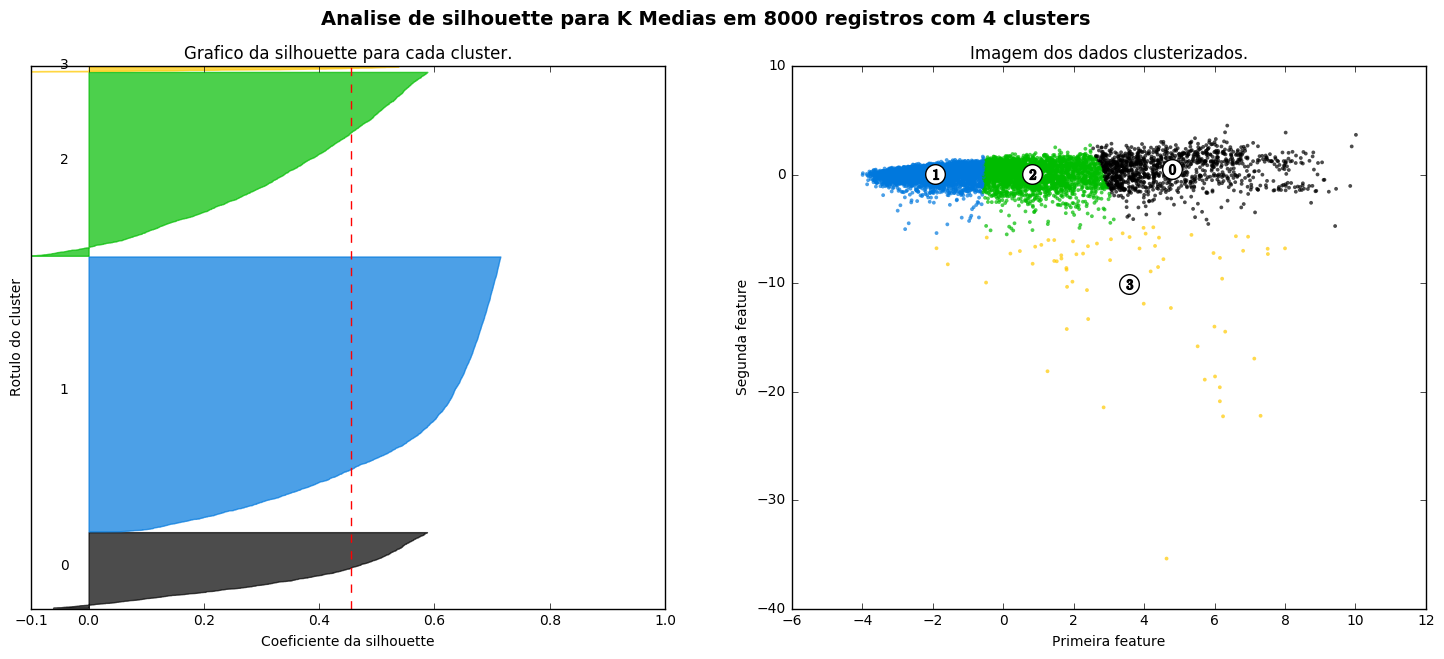
\includegraphics[width=1\textwidth]{img/silhoute4}}
\fonte{Gerado a partir do script}
\end{figure}

Para a divisão em 4 clusters, foi obtida a nota 0,4559

\begin{figure}[!ht]
\caption{Analise dos 5 clusters }
\centerline{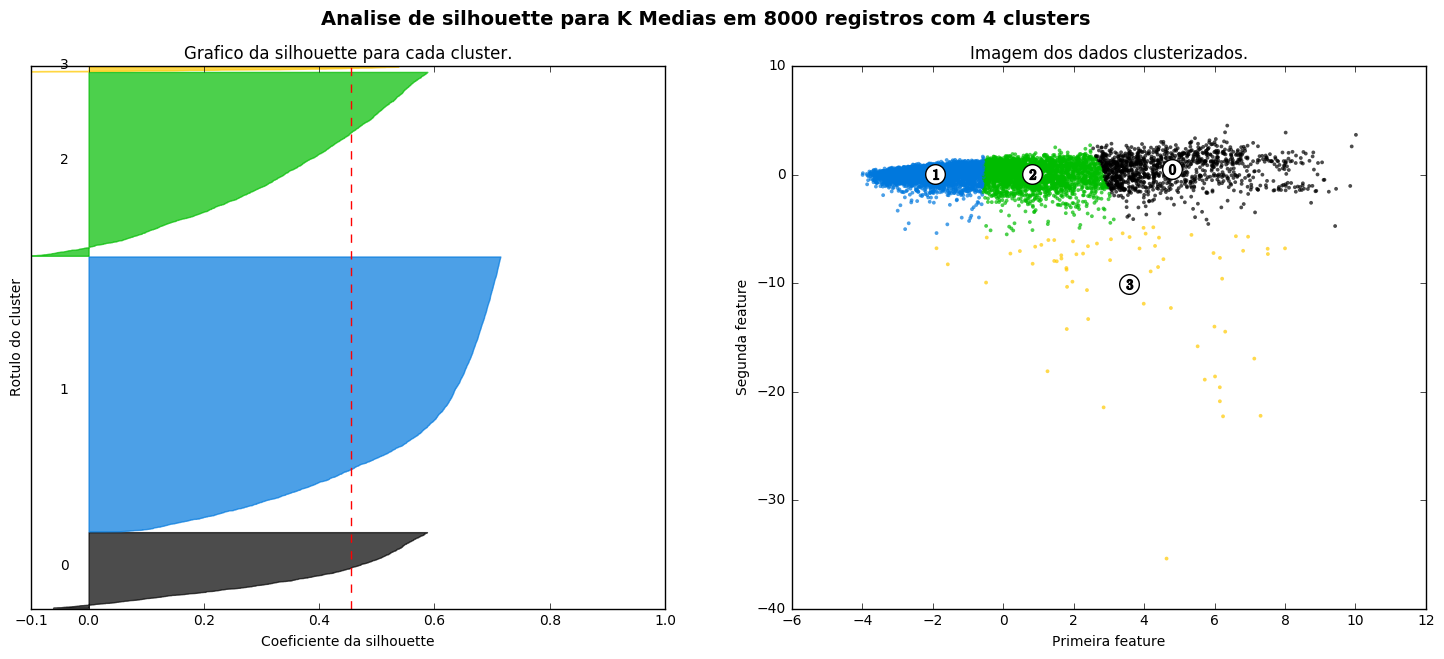
\includegraphics[width=1\textwidth]{img/silhoute4}}
\fonte{Gerado a partir do script}
\end{figure}

Para a divisão em 5 clusters, foi obtida a nota 0,4032

Podemos notar uma tendência do score cair. Contudo, maior o score, melhor. Dessa forma, há um indício de que uma boa clusterização seja com 2 centróides.



\subsection{Regressão Logística}


Também conhecida como matriz de erros, a confusion matrix é uma representação visual dos erros ocorridos durante o processamento do algoritmo. As linhas representam a classe que o dado pertence e a coluna representa a classificação gerada durante o processo. Quando um registro não está dentro da diagonal principal, significa que o algoritmo fez uma classificação diferente do que foi esperado.

\begin{figure}[!ht]
\caption{Confusion Matrix}
\centerline{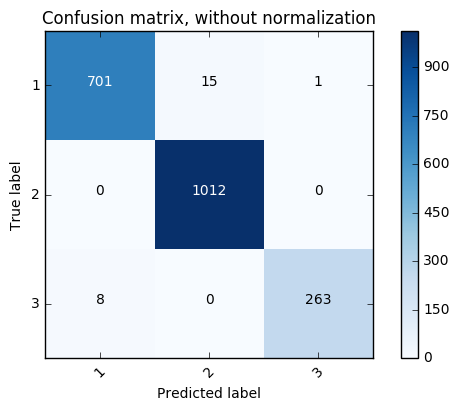
\includegraphics[width=.7\textwidth]{img/confusionMatrix}}
\fonte{Gerado a partir do script}
\end{figure}


Para o caso do Loan Club, podemos notar que a função gerada pela regressão logística possui um indíce de acurácia alto.

\subsection{Random Forest}

A árvore de classificação para 3 clusters é essa

\begin{figure}[!ht]
\caption{Estrutura da arvore de decisao}
\centerline{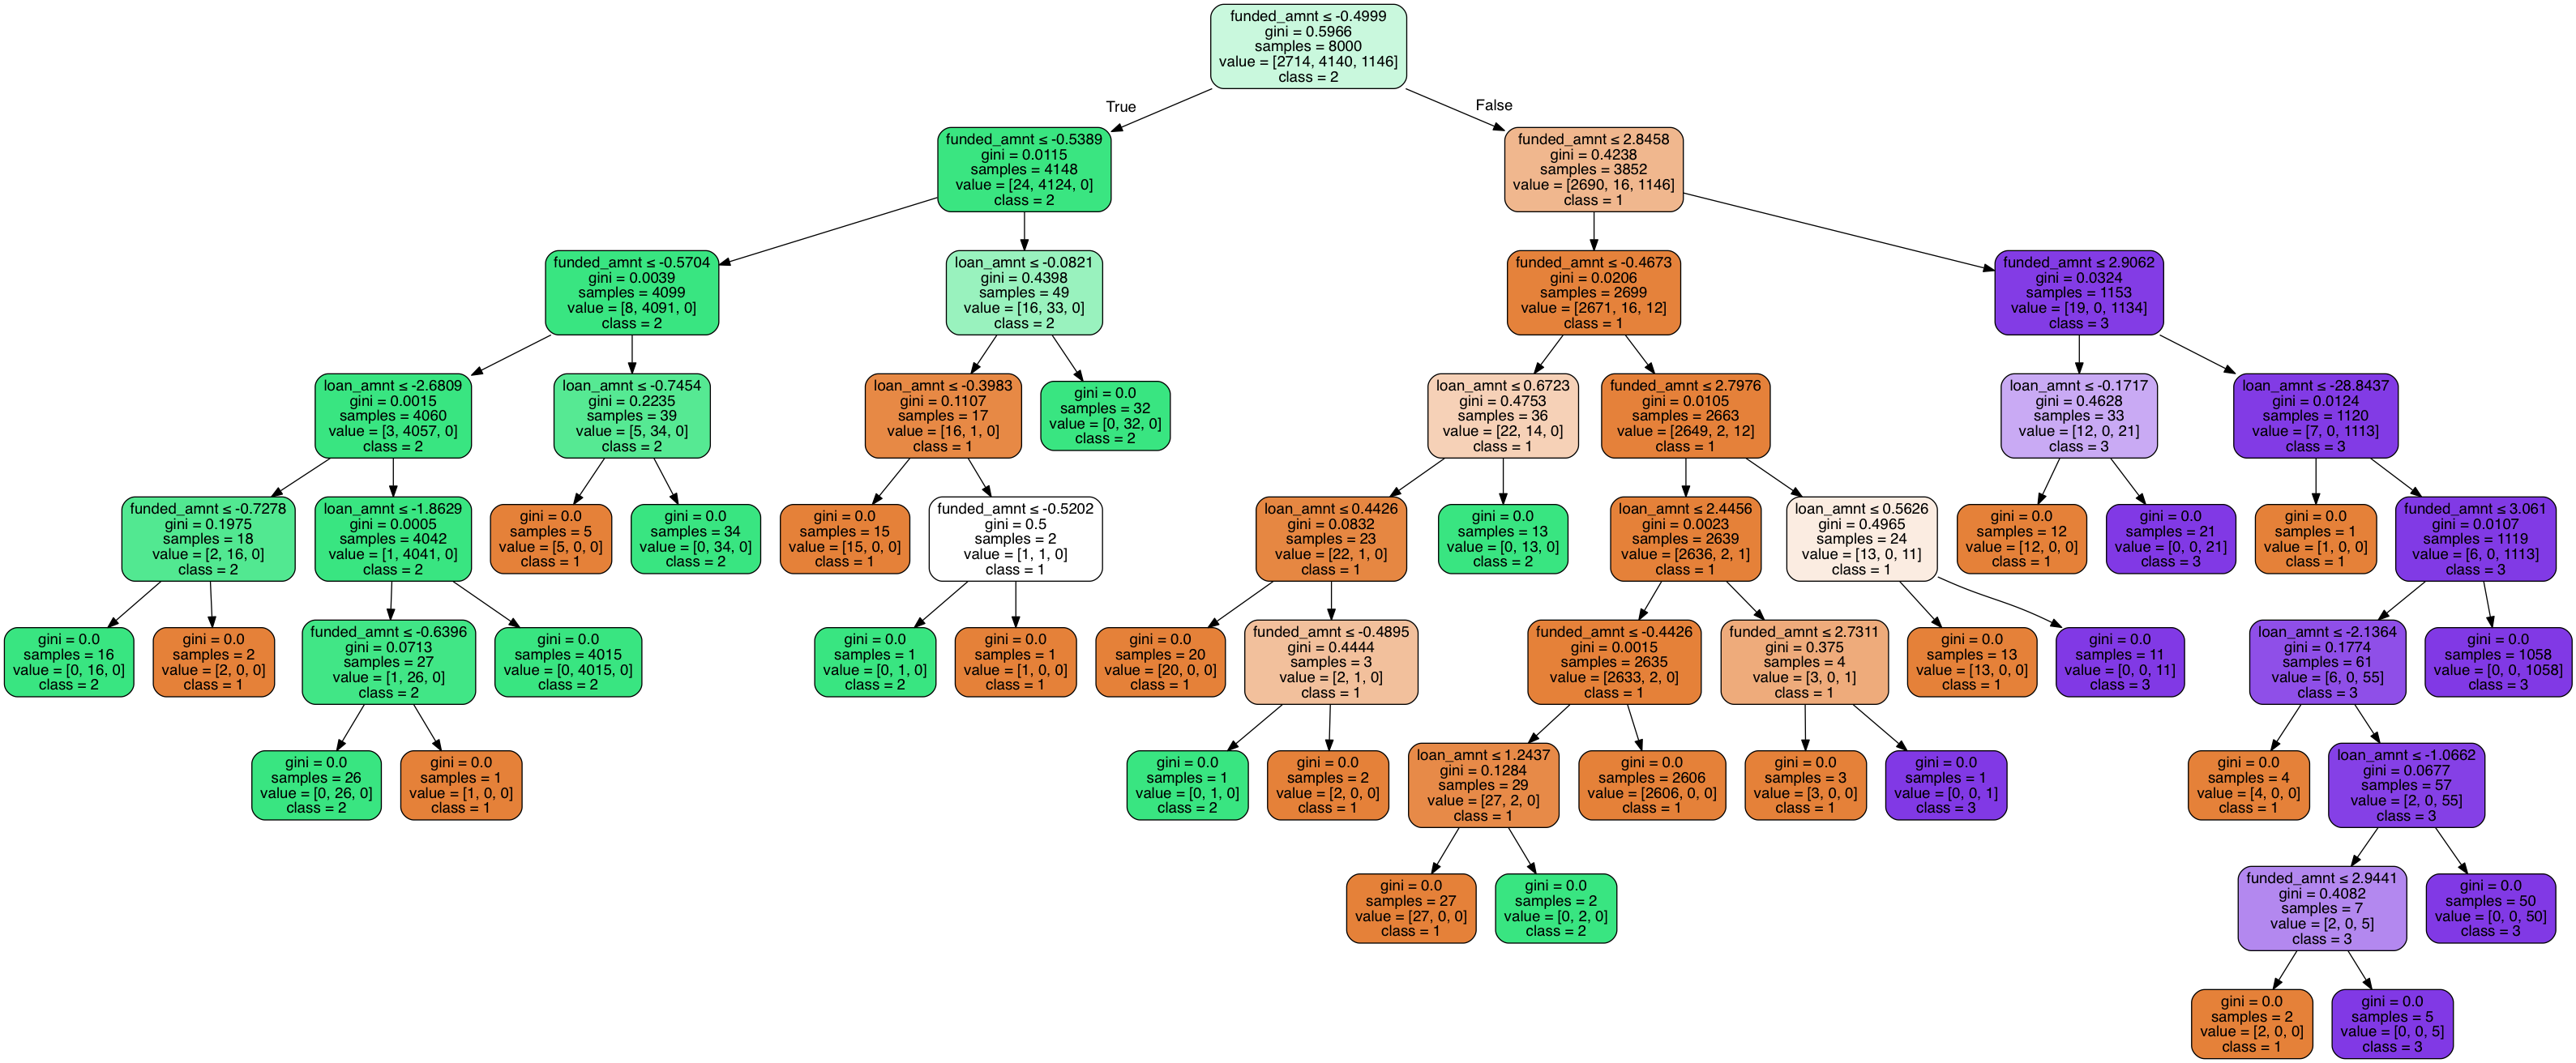
\includegraphics[width=1.05\textwidth]{img/loan}}
\fonte{Gerado a partir do script}
\end{figure}


\begin{figure}[!ht]
\caption{Features mais relevantes}
\centerline{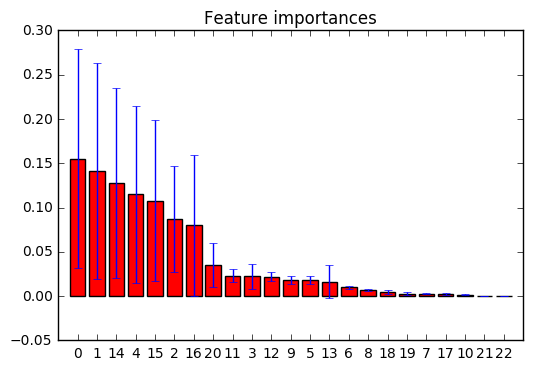
\includegraphics[width=.7\textwidth]{img/tree-most-important-features}}
\fonte{Gerado a partir do script}
\end{figure}

\lstinputlisting[language=Python, firstline=37, lastline=45]{
load_data.py
}




 \label{tab:daypack}
    \begin{tabularx}{\textwidth}{p{.3\textwidth}X}
    \caption{Tabela de campos disponíveis em Loan Club}\\
    \toprule
    \textbf{Coluna} & \textbf{Descrição} \\[6pt]
    \midrule
    \endhead

addr\textunderscore state & The state provided by the borrower in the loan application\\
annual\textunderscore inc & The self-reported annual income provided by the borrower during registration.\\
annual\textunderscore inc\textunderscore joint & The combined self-reported annual income provided by the co-borrowers during registration\\
application\textunderscore type & Indicates whether the loan is an individual application or a joint application with two co-borrowers\\
collection\textunderscore recovery\textunderscore fee & post charge off collection fee\\
collections\textunderscore 12\textunderscore mths\textunderscore ex\textunderscore med & Number of collections in 12 months excluding medical collections\\
delinq\textunderscore 2yrs & The number of 30+ days past-due incidences of delinquency in the borrower's credit file for the past 2 years\\
desc & Loan description provided by the borrower\\
dti & A ratio calculated using the borrower’s total monthly debt payments on the total debt obligations, excluding mortgage and the requested LC loan, divided by the borrower’s self-reported monthly income.\\
dti\textunderscore joint & A ratio calculated using the co-borrowers' total monthly payments on the total debt obligations, excluding mortgages and the requested LC loan, divided by the co-borrowers' combined self-reported monthly income\\
earliest\textunderscore cr\textunderscore line & The month the borrower's earliest reported credit line was opened\\
emp\textunderscore length & Employment length in years. Possible values are between 0 and 10 where 0 means less than one year and 10 means ten or more years. \\
emp\textunderscore title & The job title supplied by the Borrower when applying for the loan.*\\
fico\textunderscore range\textunderscore high & The upper boundary range the borrower’s FICO at loan origination belongs to.\\
fico\textunderscore range\textunderscore low & The lower boundary range the borrower’s FICO at loan origination belongs to.\\
funded\textunderscore amnt & The total amount committed to that loan at that point in time.\\
funded\textunderscore amnt\textunderscore inv & The total amount committed by investors for that loan at that point in time.\\
grade & LC assigned loan grade\\
home\textunderscore ownership & The home ownership status provided by the borrower during registration. Our values are: RENT, OWN, MORTGAGE, OTHER.\\
id & A unique LC assigned ID for the loan listing.\\
initial\textunderscore list\textunderscore status & The initial listing status of the loan. Possible values are – W, F\\
inq\textunderscore last\textunderscore 6mths & The number of inquiries in past 6 months (excluding auto and mortgage inquiries)\\
installment & The monthly payment owed by the borrower if the loan originates.\\
int\textunderscore rate & Interest Rate on the loan\\
is\textunderscore inc\textunderscore v & Indicates if income was verified by LC, not verified, or if the income source was verified\\
issue\textunderscore d & The month which the loan was funded\\
last\textunderscore credit\textunderscore pull\textunderscore d & The most recent month LC pulled credit for this loan\\
last\textunderscore fico\textunderscore range\textunderscore high & The upper boundary range the borrower’s last FICO pulled belongs to.\\
last\textunderscore fico\textunderscore range\textunderscore low & The lower boundary range the borrower’s last FICO pulled belongs to.\\
last\textunderscore pymnt\textunderscore amnt & Last total payment amount received\\
last\textunderscore pymnt\textunderscore d & Last month payment was received\\
loan\textunderscore amnt & The listed amount of the loan applied for by the borrower. If at some point in time, the credit department reduces the loan amount, then it will be reflected in this value.\\
loan\textunderscore status & Current status of the loan\\
member\textunderscore id & A unique LC assigned Id for the borrower member.\\
mths\textunderscore since\textunderscore last\textunderscore delinq & The number of months since the borrower's last delinquency.\\
mths\textunderscore since\textunderscore last\textunderscore major\textunderscore derog & Months since most recent 90-day or worse rating\\
mths\textunderscore since\textunderscore last\textunderscore record & The number of months since the last public record.\\
next\textunderscore pymnt\textunderscore d & Next scheduled payment date\\
open\textunderscore acc & The number of open credit lines in the borrower's credit file.\\
out\textunderscore prncp & emaining outstanding principal for total amount funded\\
out\textunderscore prncp\textunderscore inv & Remaining outstanding principal for portion of total amount funded by investors\\
policy\textunderscore code & "publicly available policy\textunderscore code=1\\
new products not publicly available policy\textunderscore code=2"\\
pub\textunderscore rec & Number of derogatory public records\\
purpose & A category provided by the borrower for the loan request. \\
pymnt\textunderscore plan & Indicates if a payment plan has been put in place for the loan\\
recoveries & post charge off gross recovery\\
revol\textunderscore bal & Total credit revolving balance\\
revol\textunderscore util & Revolving line utilization rate, or the amount of credit the borrower is using relative to all available revolving credit.\\
sub\textunderscore grade & LC assigned loan subgrade\\
term & The number of payments on the loan. Values are in months and can be either 36 or 60.\\
title & The loan title provided by the borrower\\
total\textunderscore acc & The total number of credit lines currently in the borrower's credit file\\
total\textunderscore pymnt & Payments received to date for total amount funded\\
total\textunderscore pymnt\textunderscore inv & Payments received to date for portion of total amount funded by investors\\
total\textunderscore rec\textunderscore int & Interest received to date\\
total\textunderscore rec\textunderscore late\textunderscore fee & Late fees received to date\\
total\textunderscore rec\textunderscore prncp & Principal received to date\\
verified\textunderscore status\textunderscore joint & Indicates if the co-borrowers' joint income was verified by LC, not verified, or if the income source was verified\\
zip\textunderscore code & The first 3 numbers of the zip code provided by the borrower in the loan application.\\
open\textunderscore acc\textunderscore 6m & Number of open trades in last 6 months\\
open\textunderscore il\textunderscore 6m & Number of currently active installment trades\\
open\textunderscore il\textunderscore 12m & Number of installment accounts opened in past 12 months\\
open\textunderscore il\textunderscore 24m & Number of installment accounts opened in past 24 months\\
mths\textunderscore since\textunderscore rcnt\textunderscore il & Months since most recent installment accounts opened\\
total\textunderscore bal\textunderscore il & Total current balance of all installment accounts\\
il\textunderscore util & Ratio of total current balance to high credit/credit limit on all install acct\\
open\textunderscore rv\textunderscore 12m & Number of revolving trades opened in past 12 months\\
open\textunderscore rv\textunderscore 24m & Number of revolving trades opened in past 24 months\\
max\textunderscore bal\textunderscore bc & Maximum current balance owed on all revolving accounts\\
all\textunderscore util & Balance to credit limit on all trades\\
total\textunderscore rev\textunderscore hi\textunderscore lim & Total revolving high credit/credit limit\\
inq\textunderscore fi & Number of personal finance inquiries\\
total\textunderscore cu\textunderscore tl & Number of finance trades\\
inq\textunderscore last\textunderscore 12m & Number of credit inquiries in past 12 months\\
acc\textunderscore now\textunderscore delinq & The number of accounts on which the borrower is now delinquent.\\
tot\textunderscore coll\textunderscore amt & Total collection amounts ever owed \\
tot\textunderscore cur\textunderscore bal & Total current balance of all accounts \\

\bottomrule

\end{tabularx}
% ---
% primeiro capitulo de Resultados
% ---
%\chapter{Lectus lobortis condimentum}
% ---

% ---
%\section{Vestibulum ante ipsum primis in faucibus orci luctus et ultrices
%posuere cubilia Curae}
% ---

%\lipsum[21-22]

% ---
% segundo capitulo de Resultados
% ---
%\chapter{Nam sed tellus sit amet lectus urna ullamcorper tristique interdum
%elementum}
% ---

% ---
%\section{Pellentesque sit amet pede ac sem eleifend consectetuer}
% ---

%\lipsum[24]

% ----------------------------------------------------------
% Finaliza a parte no bookmark do PDF
% para que se inicie o bookmark na raiz
% e adiciona espaço de parte no Sumário
% ----------------------------------------------------------
%\phantompart